\section{HVAC Controllers }\label{hvac-controllers}

\subsection{Control Valve for Water-Based Air System Coils}\label{control-valve-for-water-based-air-system-coils}

The input object Controller:WaterCoil provides a simple controller model for adjusting water flow rates to meet the desired air side conditions. It is really a solution inverter. For a water coil the simulation cannot be inverted where the mass flow rate of the water through the coil can be solved directly given an air temperature. Thus, this ``controller'' will numerically step through all of the water flow possibilities by a root finding technique until the mass flow rate is determined to meet the specified outlet air temperature within a specified user tolerance.

\subsubsection{Model Description}\label{model-description-012}

The figure below illustrates the use of a simple controller used with a central chilled water coil (control variable Temperature). The controller reads the desired temperature setpoint from the control node (established by a SetpointManager) and modulates the chilled water flow rate at the actuator node in order to meet the desired supply (coil outlet) air temperature.

 % fig 190
\begin{figure}[hbtp]
\centering
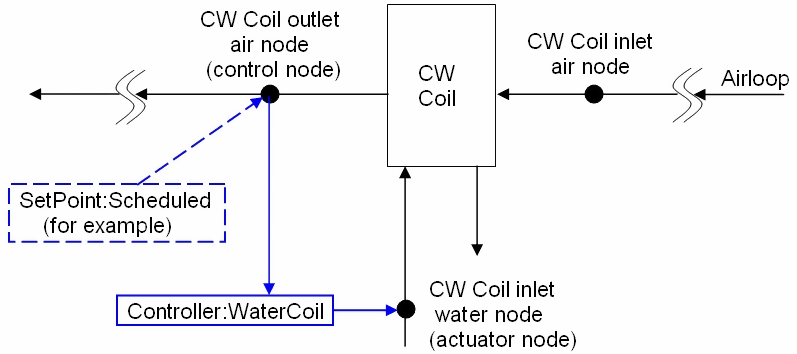
\includegraphics[width=0.9\textwidth, height=0.9\textheight, keepaspectratio=true]{media/image4384.png}
\caption{Controller:WaterCoil used with Central Chilled Water Coil \protect \label{fig:controller-watercoil-used-with-central}}
\end{figure}

In this case, the controller simply senses the temperature at the control node and compares this value with the desired temperature setpoint. If the sensed temperature is above the desired setpoint temperature, the chilled water flow rate is increased. This controller may be used for both chilled water and hot water coils. The action parameter input is set to REVERSE for chilled water cooling coils and NORMAL for hot water heating coils.

The simple controller may also be used to control both high temperature and high humidity levels by controlling the water flow rate through a chilled water coil. Setting the controller's control variable to TemperatureAndHumidityRatio enables this feature. In this case, the controller monitors two setpoint values, one for temperature control and the other for high humidity control. Note that two setpoint managers must be used to establish these setpoints as shown in the figure below. The limiting case for either temperature or high humidity control (i.e., the minimum supply air temperature required to meet both setpoints) is used for controlling the water flow rate through the chilled water coil. If high humidity control is the limiting case then colder supply air will be delivered by the cooling coil to achieve proper dehumidification and some form of air reheat may be required to avoid overcooling of the zones being served by this air loop.

\begin{figure}[hbtp] % fig 191
\centering
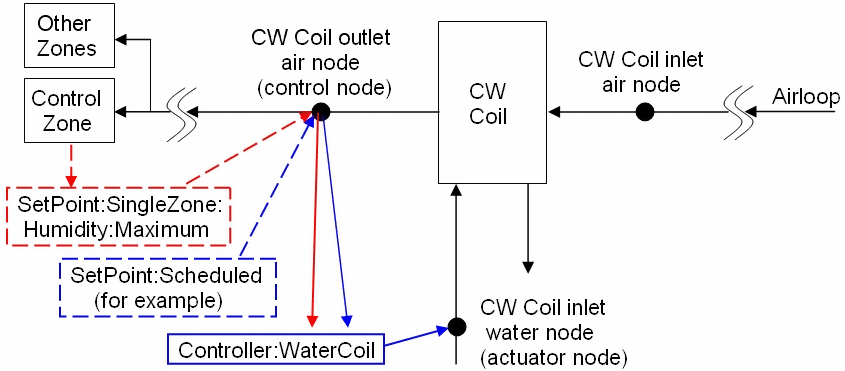
\includegraphics[width=0.9\textwidth, height=0.9\textheight, keepaspectratio=true]{media/image4385.png}
\caption{Two Setpoint managers used in Controller:WaterCoil \protect \label{fig:two-setpoint-managers-used-in-controller}}
\end{figure}

When the control variable TemperatureAndHumidityRatio is used, the controller modulates water flow through a chilled water coil to meet both a temperature and a humidity ratio setpoint. These two setpoints are placed on the control node by setpoint managers.

The model first calculates the approach temperature using the dry-bulb temperature and dewpoint temperature of the air leaving the water coil:

\begin{equation}
{T_{dp}} = {\rm{PsyTdpFnWPb}}\left( {{\omega_{SA}},P} \right)
\end{equation}

\begin{equation}
{T_{approach}} = {T_{SA}} - {T_{dp}}
\end{equation}

where:

\({T_{approach}}\) is the approach temperature (\(^{\circ}\)C)

\({\omega_{SA}}\) is the supply (outlet) air humidity ratio (kg/kg)

\(P\) is the outdoor barometric pressure (Pa)

\({T_{dp}}\) is the supply (outlet) air dewpoint temperature (\(^{\circ}\)C)

\({T_{SA}}\) is the supply (outlet) air dry-bulb temperature (\(^{\circ}\)C)

\({\rm{PsyTdpFnWPb}}\) is the EnergyPlus psychrometric function, returns dewpoint temperature given humidity ratio and barometric pressure.

The supply air dewpoint temperature required to meet the humidity ratio setpoint (placed on the control node by SetpointManager:SingleZone:Humidity:Maximum, SetpointManager:MultiZone:MaximumHumidity:Average~ or SetpointManager:MultiZone:Humidity:Maximum) is then calculated as a function of the humidity ratio setpoint and barometric pressure as follows:

\begin{equation}
{T_{dp,SP}} = {\rm{PsyTdpFnWPb}}\left( {{\omega_{SP}},P} \right)
\end{equation}

where:

\({T_{dp,SP}}\) is the dewpoint temperature corresponding to \emph{w\(_{SP}\)} (\(^{\circ}\)C)

\({\omega_{SP}}\) is the humidity ratio setpoint (kg/kg).

In order for the dewpoint temperature of the coil's supply (outlet) air to reach \({T_{dp,SP}}\) the dry-bulb temperature of air leaving the cooling coil must be at \({T_{dp,SP}} + {T_{approach}}\):

\begin{equation}
{T_{HR,SP}} = {T_{dp,SP}} + {T_{approach}}
\end{equation}

where: \({T_{HR,SP}}\) is the supply air dry-bulb temperature setpoint required to achieve the specified humidity ratio setpoint (\(^{\circ}\)C).

The supply air temperature setpoint required to achieve the specified humidity ratio setpoint is then compared to the setpoint temperature required for zone temperature control, and the minimum of these two setpoint values is used as the setpoint temperature for controlling the chilled water coil.

\begin{equation}
{T_{SP}} = MIN\left( {{T_{Temp,SP}},{T_{HR,SP}}} \right)
\end{equation}

where:

\({T_{SP}}\) = chilled water coil supply air temperature setpoint (\(^{\circ}\)C)

\({T_{Temp,SP}}\) = supply air temperature setpoint required for zone temperature control (\(^{\circ}\)C).

As described previously, the controller varies the chilled water flow rate through the coil using a root finding technique until the actual supply air temperature reaches \emph{T\(_{sp}\)}within the specified tolerance:

\begin{equation}
{T_{Actual}} - {T_{SP}} \le Controller~Convergence~Tolerance
\end{equation}

where \({T_{Actual}}\) is the actual air temperature leaving the cooling coil (\(^{\circ}\)C).

\subsection{Outdoor Air Damper Controller for Air Systems}\label{outdoor-air-damper-controller-for-air-systems}

When the heat exchanger assisted cooling coil is used with a furnace or unitary system (ref. AirLoopHVAC:Unitary:Furnace:HeatCool or AirLoopHVAC:UnitaryHeatCool) or DX system (ref. CoilSystem:Cooling:DX) located in an air loop (or DX system used in an outside air system), an economizer function may be customized as necessary. For economizer control, an outdoor air controller (ref. Controller:OutdoorAir) is used to define the economizer control inputs and determine when economizer mode is active. The heat exchanger (ref. HeatExchanger:*) object provides an economizer lockout feature which disables heat recovery any time the economizer is active. This feature can be turned on and off using the heat exchanger lockout input. Heat exchanger assisted cooling coils used with the zone equipment described below disregard this economizer control feature. The heat recovery bypass control input may also be used to selectively control heat recovery.

\subsubsection{Inputs}\label{inputs}

\begin{itemize}
\item
  Controller Name
\item
  Relief air node
\item
  Return air node
\item
  Control node (the mixed air node)
\item
  Actuated node (the outside air inlet node)
\item
  Minimum outside air flow rate (at design) (m\(^{3}\)/s)
\item
  Maximum outside air flow rate~ (\({\dot V_{oa,max }}\)) (m\(^{3}\)/s)
\item
  EconomizerChoice: \emph{FixedDryBulb} \textbar{} \emph{FixedEnthalpy} \textbar{} \emph{~DifferentialDryBulb~} \textbar{} \emph{~DifferentialEnthalpy} \textbar{} \emph{~~ElectronicEnthalpy} \textbar{} \emph{~~FixedDewPointAndDryBulb~~~} \textbar{} \emph{DifferentialDryBulbAndEnthalpy~} \textbar{} \emph{NoEconomizer}
\item
  Bypasschoice: \emph{MinimumFlowWithBypass} \textbar{} \emph{ModulateFlow}
\item
  High temperature limit (\({T_{high}}\)) (\(^{\circ}\)C)
\item
  High specific enthalpy limit (\({h_{high}}\)) (J/kg)
\item
  High dewpoint temperature limit (\({T_{DP,high}}\)) (\(^{\circ}\)C)
\item
  Electronic Enthalpy limit (quadratic or cubic curve object)
\item
  Low temperature limit (\({T_{low}}\)) (\(^{\circ}\)C)
\item
  Lockout: \emph{LockoutWithHeating} \textbar{} \emph{LockoutWithCompressor}
\item
  MinimumLimit: \emph{FixedMinimum} \textbar{} \emph{ProportionalMinimum}
\item
  Minimum Outdoor Air Schedule (schedule values multiply the minimum outside air flow rate)
\item
  Minimum Fraction of Outdoor Air Schedule(schedule values sets the limit on minimum outside air fraction)
\item
  Maximum Fraction of Outdoor Air Schedule(schedule values sets the maximum outside air fraction possible in the system)
\item
  Name of Controller:MechanicalVentilation object
\item
  Time-of-day economizer control schedule (economizer active when schedule values are greater than 0)
\item
  High humidity control flag: \emph{Yes} \textbar{} \emph{No}
\item
  Humidistat control zone name (zone name where humidistat is located)
\item
  Control high indoor humidity based on outdoor humidity ratio: \emph{Yes} \textbar{} \emph{No}
\item
  High humidity outside air flow ratio (this flow ratio is multiplied by the maximum outside air flow rate during periods of high indoor relative humidity)
\item
  Heat Recovery Bypass Control Type: BypassWhenWithinEconomizerLimits \textbar{} BypassWhenOAFlowGreaterThanMinimum
\end{itemize}

\subsubsection{Economizer Limits}\label{economizer-limits}

Economizer limits may be used to create single-point or multi-point controllers. The figure below shows several examples of each type of controller. Single-point economizer controllers use a single independent variable to specify the operation of the economizer. In all cases, the economizer is disabled (OFF) when the outdoor weather condition exceeds the limit. However, when a low temperature limit is used the economizer is disabled when the outdoor temperature is \emph{below} the low dry-bulb temperature limit.

Economizer limits may also be used to create multi-point controllers where two or more limits specify the economizer operating region. The economizer is disabled (OFF) if \emph{any single} multi-point economizer limit is exceeded.

\begin{figure}[hbtp] % fig 192
\centering

\includegraphics[width=0.9\textwidth, height=0.9\textheight, keepaspectratio=true]{media/image4411.png}
\caption{Economizer Limit Controls \protect \label{fig:economizer-limit-controls}}
\end{figure}

\subsubsection{Simulation}\label{simulation-000}

The simulation contains 4 steps.

\subsubsection{Step 1: Calculate the minimum outside air flow rate}\label{step-1-Calculate-the-minimum-outside-air-flow-rate}

The user inputs the minimum outside air flow rate (or it is automatically calculated by the program from the user's design inputs). This is converted to a mass flow rate \({\dot m_{oa,\min ,des}}\) using the density of dry air at 20\(^{\circ}\)C. If the economizer is on an air loop then the minimum outside air flow fraction is initialized to:

\begin{equation}
{f_{oa,\min }} = {\dot m_{oa,\min ,des}}/{\dot m_{s,des}}
\end{equation}

where \({\dot m_{s,des}}\) is the design supply air mass flow rate. If the economizer is not on an air loop the minimum outside air flow fraction is initialized to:

\begin{equation}
{f_{oa,\min }} = {\dot m_{oa,\min ,des}}/{\dot m_{oa,\max ,des}}
\end{equation}

where \({\dot m_{oa,\max ,des}}\) is the user input maximum outside air volumetric flow rate converted to mass flow rate in the same manner as for the minimum outside air flow rate. If a minimum outside air schedule has been input, \({f_{oa,\min }}\) is multiplied by the current schedule value.

\subsubsection{Step 2: Calculate an initial outside air signal}\label{step-2-Calculate-an-initial-outside-air-signal}

We now define an initial outside air signal \({S_{oa,init}}\) .

If \(\left| {{T_{_r}} - {T_{in}}} \right| > \Delta {T_{small}}\), then:

\begin{equation}
{S_{oa,init}} = ({T_r} - {T_{mix,set}})/({T_r} - {T_i})
\end{equation}

Otherwise:

if \({T_r} < {T_{mix,set}}\) and \({T_r} \ge {T_i}\), \({S_{oa,init}}\) is set to -1;

if \({T_r} < {T_{mix,set}}\) and \({T_r} < {T_i}\), \({S_{oa,init}}\) is set to 1;

if \({T_r} \ge {T_{mix,set}}\) and \({T_r} \ge {T_i}\), \({S_{oa,init}}\) is set to 1;

if \({T_r} \ge {T_{mix,set}}\) and \({T_r} < {T_i}\), \({S_{oa,init}}\) is set to -1.

Finally, \({S_{oa,init}}\) is constrained to be: \({f_{oa,\min }} \le {S_{oa,init}} \le 1\). Basically, if the outside air can not accomplish cooling, \({S_{oa,init}}\) is set to \({f_{oa,\min }}\). If it can do cooling, \({S_{oa,init}}\) is greater than the minimum outside air flow fraction but not greater than 1. Here:

\emph{T\(_{r}\)} is the return air temperature (\(^{\circ}\)C)

\emph{T\(_{i}\)} is the outside air inlet temperature (\(^{\circ}\)C)

\emph{T\(_{mix,set}\)} is the mixed air setpoint (\(^{\circ}\)C)

\emph{\(\Delta {T_{small}}\)} is a small temperature difference (\(\Delta^{\circ}\)C), equal to 0.00001.

\subsubsection{Step 3: Do the on/off and limit checks}\label{step-3-Do-the-onoff-and-limit-checks}

\begin{itemize}
\item
If \emph{EconomizerChoice} = \emph{No Economizer}, \({S_{oa,init}} = {f_{oa,\min }}\).
\item
If \({\dot V_{oa,\max }} < {\dot V_{small}}\) , \({S_{oa,init}} = {f_{oa,\min }}\) ; \({\dot V_{small}}\) is.001 m\(^{3}\)/s.
\item
If the economizer is locked out, \({S_{oa,init}} = {f_{oa,\min }}\).
\end{itemize}

Note: the above three checks also set the \emph{EconomizerOperationFlag} and \emph{HighHumidityControlFlag} to \emph{false} (economizer and high humidity control not operating).

\begin{itemize}
\item If \({T_i} > {T_{mix,set}}\), \({S_{oa,init}} = 1\).
\item If Differential dry-bulb was input as Economizer choice and \({T_i} > {T_r}\), then \({S_{oa,init}} = {f_{oa,\min }}\).
\item If Differential Enthalpy was input as Economizer choice and \({h_i} > {h_r}\) , then \({S_{oa,init}} = {f_{oa,\min }}\), where \emph{h\(_{i}\)} and \emph{h\(_{r}\)}~are the outside air inlet and return air enthalpies.
\end{itemize}

Setpoints are checked after this which include check for Fixed dry-bulb temperature~ limit, Enthalpy Limit, Dewpoint Limit and Humidity ratio limit if specified.

\begin{itemize}
\item If Differential Enthalpy was input as Economizer choice and \({h_i} > {h_r}\) , then \({S_{oa,init}} = {f_{oa,\min }}\), where \emph{h\(_{i}\)} and \emph{h\(_{r}\)}~are the outside air inlet and return air enthalpies.
\end{itemize}

Setpoints are checked after this which include check for Fixed dry-bulb temperature limit, Enthalpy Limit, Dewpoint Limit and Humidity ratio limit if specified.

\begin{itemize}
\item If a FixedDryBulb / FixedEnthalpy / FixedDewPointAndDryBulb / ElectronicEnthalpy was input as the economizer choice then the limits are checked as before.
\item Limits are checked as follows:
\begin{itemize}
\item If a high temperature limit was input and \({T_{oa}} > {T_{high}}\), \({S_{oa,init}} = {f_{oa,\min }}\); where \emph{T\(_{oa}\)} is the outside air temperature.
\item If an enthalpy limit was input and \({h_{oa}} > {h_{high}}\), \({S_{oa,init}} = {f_{oa,\min }}\); where \emph{h\(_{oa}\)} is the outside air specific enthalpy.
\item If a dewpoint temperature limit was input and \({T_{DP,OA}} > {T_{DP,high}}\), \({S_{oa,init}} = {f_{oa,\min }}\); where T\(_{DP,OA}\) is the outside air dewpoint temperature and T\(_{DP,high}\) is the dewpoint temperature limit.
\item If an electronic enthalpy curve was input and \({w_{OA}} > {w_{CurveOutput}}\), \({S_{oa,init}} = {f_{oa,\min }}\) ; where \emph{w}\(_{OA}\) is the outside air humidity ratio and \emph{w}\(_{CurveOutput}\) is the curve's humidity ratio output as a function of outdoor air dry-bulb temperature.
\end{itemize}
\item Another Economizer choice called DifferentialDryBulbAndEnthalpy checks the outside air temperature against return temperature and outside air enthalpy against return air enthalpy and also checks the setpoints.
\item If a low temperature limit was input and \({T_{oa}} < {T_{low}}\), \({S_{oa,init}} = {f_{oa,\min }}\).
\end{itemize}

Note: the above nine cases set the \emph{EconomizerOperationFlag} to \emph{false} (economizer not operating), otherwise the economizer is active.

\begin{itemize}
\item If high humidity control is specified and the zone humidistat indicates a moisture load (i.e.~zone relative humidity greater than the relative humidity setpoint), the \emph{HighHumidityOperationFlag} is set to \emph{true.} If high humidity control is based on the outdoor humidity ratio then the \emph{HighHumidityOperationFlag} is set to \emph{true} only when the outdoor air humidity ratio is less than the humidistat's zone humidity ratio. A \emph{true} HIghHumidityOperationFlag also enables economizer operation in the heat exchangers as if the economizer flag used here was also set to \emph{true} (Ref. HeatExchanger:* - field Economizer Lockout).
\end{itemize}

The economizer schedule is then checked to determine if a ``push-button'' type economizer control is used. When schedule values are greater than 0, the economizer is active (\emph{EconomizerOperationFlag} = \emph{true)}. This test overrides the economizer limit checks described above in Step 3.

\subsubsection{Step 4: Calculate the final outside air signal}\label{step-4-Calculate-the-final-outside-air-signal}

If \emph{S\(_{oa,init}\)} is greater than \({f_{oa,\min }}\) and less than 1 and the mixed air mass flow rate is greater than \({\dot m_{verysmall}}\) (\({10^{ - 30}}\) ) and night venting is not occurring and \emph{HighHumidityOperationFlag} is false, then we calculate a final outside air signal \emph{S\(_{oa}\)} by using the root solver method routine \emph{SolveRegulaFalsi} to zero the residual \({T_{mix,set}} - {T_{mix}}\) by varying the outside air mass flow rate \({S_{oa}}\cdot {\dot m_{mix}}\) . Mass and energy balance are used to obtain the mixed air humidity ratio and enthalpy from the recirculated air and outside air inlet conditions. The psychrometric function \emph{PsyTdbFnHW} is used to obtain \emph{T\(_{mix}\)} from the mixed air enthalpy and humidity ratio.

Otherwise, \({S_{oa}} = {S_{oa,init}}\).

\subsubsection{Step 5: calculate the outside air flow rate and apply final constraints}\label{step-5-calculate-the-outside-air-flow-rate-and-apply-final-constraints}

If \emph{BypassChoice} = \emph{True and HighHumidityOperationFlag = false}, \({S_{oa}} = {f_{oa,\min }}\).

If the \emph{HighHumidityOperationFlag} is \emph{true}, then:

\begin{equation}
  S_{oa} = \max\PB{f_{oa,min},OAFlowRatio_{HighRH}\frac{\dot{m}_{oa,max,des}}{\dot{m}_{mix}}}
\end{equation}

If night ventilation is occurring, \({S_{oa}} = 1\).  Note that night ventilation has priority over the above constraints.

Now, the outside air flow rate is calculated:

\begin{equation}
{m_{oa}} = {S_{oa}}*{m_{mix}}
\end{equation}

Next, calculate the outside air mass flow rate:

If EconomizerOperationFlag is true and HighHumidityOperationFlag is false, then

\begin{equation}
{\dot m_{oa}} = {S_{oa}}\cdot {\dot m_{oa,\max ,des}}
\end{equation}

Otherwise:

\begin{equation}
{\dot m_{oa}} = {S_{oa}}\cdot {\dot m_{mix}}
\end{equation}

Then the following constraints are applied:

\begin{itemize}
\item  \({\dot m_{oa}}\) ~must be greater than or equal to the air primary loop total exhaust air mass flow rate (\({\dot m_{exhaust}}\)).

\item  If \emph{MinimumLimit} = \emph{Fixed Minimum}, \({\dot m_{oa}}\) must be greater than or equal to the minimum outside air mass flow rate.

\item  If the Minimum Fraction of Outdoor Air Schedule or the Maximum Fraction of Outdoor Air Schedule is available, outside air fraction S\(_{oa}\) = \({\dot m_{oa}}\) / \({\dot m_{mix}}\) is checked against those fractions from the schedule.

\begin{equation}
S_{oa} = Maximum(Minimum~OA~fraction, S_{oa})
\end{equation}

\begin{equation}
S_{oa} = Minimum(Maximum~OA~fraction, S_{oa})
\end{equation}

\item  \({\dot m_{oa}}\) must be \(\le\) the maximum outside air mass flow rate.

\item  If there is an EMS override set \({\dot m_{oa}}\) = EMS actuated OA mass flow rate.

\item  If there is a demand limiting override set \({\dot m_{oa}}\) = Demand limiting OA mass flow rate.

\item  \({\dot m_{oa}}\) must be \(\le {\dot m_{mix}}\) .

\end{itemize}

If heat recovery bypass control is selected, the type of control determines how heat recovery is simulated. If BypassWhenWithinEconomizerLimits is selected, heat recovery is only active when the EconomizerOperationFlag is false. If BypassWhenOAFlowGreaterThanMinimum is selected \emph{and} the EconomizerOperationFlag is true \emph{and} the outside air mass flow rate is greater than the minimum flow rate, heat recovery is disabled, otherwise heat recovery is active. The heat recovery bypass control option is used to optimize heat recovery in heating mode. Heat recovery is commonly used to reduce the cooling load when outdoor conditions are higher than indoor conditions, however, when outdoor conditions are favorable the heat exchanger can be turned off and the economizer may be used to also reduce the cooling load. Economizer mode is typically involves increasing the outdoor air flow rate. At some point the outdoor air flow rate must be reduced and the heat exchanger should be turned back on to reduce or avoid an indoor heating requirement. This option will typically be used with some form of supply air temperature control used with the heat recovery equipment (Ref. HeatExchanger).

\subsubsection{Step 6: Set the relief air mass flow rate}\label{step-6-Set-the-relief-air-mass-flow-rate}

\begin{equation}
{\dot m_{relief}} = \max (0,{\dot m_{oa}} - {\dot m_{exhaust}})
\end{equation}

\subsection{Outdoor Air Damper Controller for Zone Energy Recovery Ventilator}\label{outdoor-air-damper-controller-for-zone-energy-recovery-ventilator}

The stand alone energy recovery ventilator (ERV) controller is used solely in conjunction with a stand alone energy recovery ventilator (see figure below).

\begin{figure}[hbtp] % fig 193
\centering
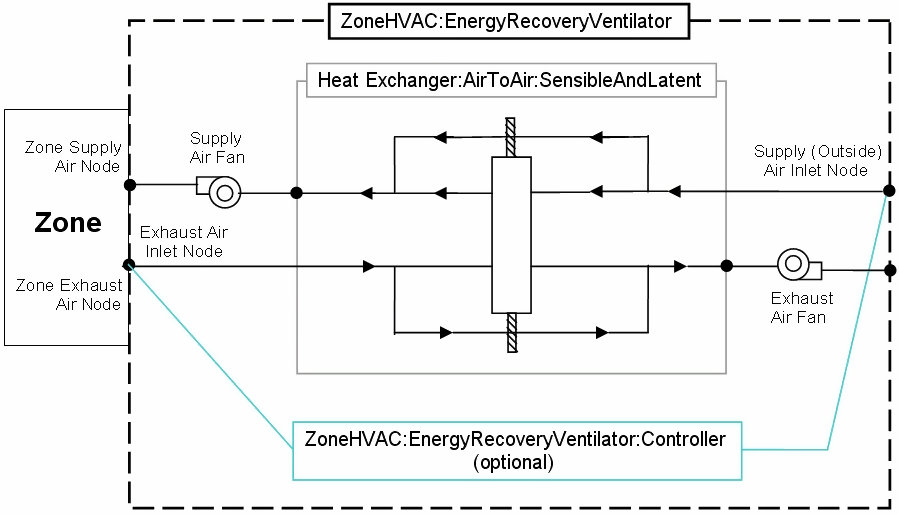
\includegraphics[width=0.9\textwidth, height=0.9\textheight, keepaspectratio=true]{media/image4482.png}
\caption{Schematic of the ZoneHVAC:EnergyRecoveryVentilator Compound Object \protect \label{fig:schematic-of-the-zonehvac}}
\end{figure}

This controller object mimics virtually all of the control logic available for a conventional air-side economizer as embodied in the object Controller:OutdoorAir. However, this controller is only used with the stand alone energy recovery ventilator object (dedicated to serving a single zone, without a traditional air distribution system) while the Controller:OutdoorAir is used with systems that utilize an air loop to provide conditioned air to one or more zones. The purpose of this controller is to signal the object HeatExchanger:AirToAir:SensibleAndLatent that favorable conditions are available for free cooling and heat exchange should be suspended (i.e., air flow is fully bypassed around a fixed-plate heat exchanger or the rotation of a rotary heat exchanger is stopped). A time-of-day schedule may also be used to simulate a ``push-button'' type economizer. The air flow rate through the stand alone ERV remains the same regardless of whether the controller is signaling for economizer (free cooling) operation or not. In this way, this controller is very similar to Controller:OutdoorAir with the field Economizer Control Action Type set to ``MinimumFlowWithBypass''. However, the supply and exhaust air flow rates may be modified in response to a high indoor humidity condition (i.e., when the zone relative humidity is ``predicted'' to exceed the setpoint, at times the actual zone relative humidity may be slightly below the setpoint. Ref. Zone/Sys Moisture Load Rate Predicted.) and works in a similar fashion to the outside air controller where the air flow rates are adjusted based on a user specified air flow \emph{ratio}.

\subsubsection{Controller Logic}\label{controller-logic}

In many ways, the logic for this controller follows that established for the object Controller:OutdoorAir. Nearly the same computations (source code) are used for this controller as for Controller:OutdoorAir, except the addition of a few calculations that are unique for this stand alone ERV controller. Refer to the \emph{Simulation} discussion for the outdoor air controller to review the calculation procedure. In some instances local variables used in the Controller:OutdoorAir computations are set to specific values for ZoneHVAC:EnergyRecoveryVentilator:Controller to allow the same computations and logic to be used for both controllers. The logic that is being applied for ZoneHVAC:EnergyRecoveryVentilator:Controller is presented below.

As explained above the controller senses when air conditions are such that heat exchange by the air-to-air heat exchanger should be suspended to provide free cooling to the zone, thereby reducing the amount of mechanical cooling that needs to be provided by other equipment. The inputs for this controller specify temperature and/or enthalpy conditions that are used to trigger economizer operation. An economizer lockout input is provided in the heat exchanger object and is used for customizing heat exchanger performance during economizer operation. Heat exchange is suspended only if the heat exchanger's economizer lockout input is set to Yes.

The user can enter a high and low temperature limit for economizer operation. When the supply inlet (outdoor) air is between these two values, heat exchange is suspended while air flow rates remain unchanged. This logic represents a conventional single-point temperature economizer control. If the user wishes to model differential temperature control, EXHAUST AIR TEMP LIMIT should be specified in the proper input field. In this case, heat exchange is suspended whenever the temperature of the exhaust air is greater than the temperature of the outdoor air. The user still needs to set the low temperature limit to restart the heat exchange process when the outdoor temperature falls too low.

A high dewpoint temperature limit may also be specified. When the supply inlet (outdoor) air is below this limit, heat exchange is suspended while air flow rates remains unchanged. The user still needs to set the low temperature limit to restart the heat exchange process when the outdoor temperature falls too low.

Similar logic can be used with air enthalpy. The user can enter a high enthalpy limit, and heat exchange between the supply and exhaust air streams will be suspended when the outdoor air enthalpy falls below this value. This logic represents single-point enthalpy economizer control. If the user wishes to model differential enthalpy control, EXHAUST AIR ENTHALPY LIMIT should be specified in the proper input field. Regardless of modeling single-point enthalpy or differential enthalpy control, the user still needs to set the low temperature limit to restart the heat exchange process when the outdoor temperature falls too low.

The user may also specify an electronic enthalpy curve object to represent a variable enthalpy controller. A quadratic or cubic curve is used in this case. The output of this curve would represent the maximum outdoor humidity ratio allowed as a function of outdoor dry-bulb temperature.

The air flow rates through the stand alone ERV may also be modified based on a high indoor relative humidity condition. The change in air flow rates may occur at any time the indoor relative humidity is high or when the indoor relative humidity is high \emph{and} the outdoor humidity ratio is lower than the indoor humidity ratio. This control mode modifies the air flow rates according to the user specified high humidity outside air flow ratio. When high humidity control is active, heat exchange is suspended in the same manner as if an economizer were used and, as with economizer operation, heat exchange is suspended only if the heat exchanger's economizer lockout input is set to Yes.

The model is flexible, and checks all limits established by the user in the object's input data. The model initially assumes that heat exchange should be suspended, and then checks each one of the limits that the user has set (single-point temperature, differential temperature, single-point enthalpy and differential point enthalpy, single-point dewpoint or electronic (variable) enthalpy). If any of the limits entered by the user is exceeded, then economizer operation is terminated and heat exchange between the supply and exhaust air streams is modeled.
